% Options for packages loaded elsewhere
\PassOptionsToPackage{unicode}{hyperref}
\PassOptionsToPackage{hyphens}{url}
\PassOptionsToPackage{dvipsnames,svgnames,x11names}{xcolor}
%
\documentclass[
  letterpaper,
  DIV=11,
  numbers=noendperiod]{scrartcl}

\usepackage{amsmath,amssymb}
\usepackage{iftex}
\ifPDFTeX
  \usepackage[T1]{fontenc}
  \usepackage[utf8]{inputenc}
  \usepackage{textcomp} % provide euro and other symbols
\else % if luatex or xetex
  \usepackage{unicode-math}
  \defaultfontfeatures{Scale=MatchLowercase}
  \defaultfontfeatures[\rmfamily]{Ligatures=TeX,Scale=1}
\fi
\usepackage{lmodern}
\ifPDFTeX\else  
    % xetex/luatex font selection
  \setmainfont[]{Atkinson Hyperlegible}
  \setsansfont[]{Atkinson Hyperlegible}
  \setmonofont[]{Fira Code}
\fi
% Use upquote if available, for straight quotes in verbatim environments
\IfFileExists{upquote.sty}{\usepackage{upquote}}{}
\IfFileExists{microtype.sty}{% use microtype if available
  \usepackage[]{microtype}
  \UseMicrotypeSet[protrusion]{basicmath} % disable protrusion for tt fonts
}{}
\makeatletter
\@ifundefined{KOMAClassName}{% if non-KOMA class
  \IfFileExists{parskip.sty}{%
    \usepackage{parskip}
  }{% else
    \setlength{\parindent}{0pt}
    \setlength{\parskip}{6pt plus 2pt minus 1pt}}
}{% if KOMA class
  \KOMAoptions{parskip=half}}
\makeatother
\usepackage{xcolor}
\setlength{\emergencystretch}{3em} % prevent overfull lines
\setcounter{secnumdepth}{-\maxdimen} % remove section numbering
% Make \paragraph and \subparagraph free-standing
\ifx\paragraph\undefined\else
  \let\oldparagraph\paragraph
  \renewcommand{\paragraph}[1]{\oldparagraph{#1}\mbox{}}
\fi
\ifx\subparagraph\undefined\else
  \let\oldsubparagraph\subparagraph
  \renewcommand{\subparagraph}[1]{\oldsubparagraph{#1}\mbox{}}
\fi


\providecommand{\tightlist}{%
  \setlength{\itemsep}{0pt}\setlength{\parskip}{0pt}}\usepackage{longtable,booktabs,array}
\usepackage{calc} % for calculating minipage widths
% Correct order of tables after \paragraph or \subparagraph
\usepackage{etoolbox}
\makeatletter
\patchcmd\longtable{\par}{\if@noskipsec\mbox{}\fi\par}{}{}
\makeatother
% Allow footnotes in longtable head/foot
\IfFileExists{footnotehyper.sty}{\usepackage{footnotehyper}}{\usepackage{footnote}}
\makesavenoteenv{longtable}
\usepackage{graphicx}
\makeatletter
\def\maxwidth{\ifdim\Gin@nat@width>\linewidth\linewidth\else\Gin@nat@width\fi}
\def\maxheight{\ifdim\Gin@nat@height>\textheight\textheight\else\Gin@nat@height\fi}
\makeatother
% Scale images if necessary, so that they will not overflow the page
% margins by default, and it is still possible to overwrite the defaults
% using explicit options in \includegraphics[width, height, ...]{}
\setkeys{Gin}{width=\maxwidth,height=\maxheight,keepaspectratio}
% Set default figure placement to htbp
\makeatletter
\def\fps@figure{htbp}
\makeatother
\newlength{\cslhangindent}
\setlength{\cslhangindent}{1.5em}
\newlength{\csllabelwidth}
\setlength{\csllabelwidth}{3em}
\newlength{\cslentryspacingunit} % times entry-spacing
\setlength{\cslentryspacingunit}{\parskip}
\newenvironment{CSLReferences}[2] % #1 hanging-ident, #2 entry spacing
 {% don't indent paragraphs
  \setlength{\parindent}{0pt}
  % turn on hanging indent if param 1 is 1
  \ifodd #1
  \let\oldpar\par
  \def\par{\hangindent=\cslhangindent\oldpar}
  \fi
  % set entry spacing
  \setlength{\parskip}{#2\cslentryspacingunit}
 }%
 {}
\usepackage{calc}
\newcommand{\CSLBlock}[1]{#1\hfill\break}
\newcommand{\CSLLeftMargin}[1]{\parbox[t]{\csllabelwidth}{#1}}
\newcommand{\CSLRightInline}[1]{\parbox[t]{\linewidth - \csllabelwidth}{#1}\break}
\newcommand{\CSLIndent}[1]{\hspace{\cslhangindent}#1}

\usepackage{fancyhdr}
\pagestyle{fancy}
\fancyfoot[C]{\thepage}
\renewcommand{\headrulewidth}{0.4pt}
\renewcommand{\footrulewidth}{0.4pt}
\KOMAoption{captions}{tableheading}
\makeatletter
\@ifpackageloaded{tcolorbox}{}{\usepackage[skins,breakable]{tcolorbox}}
\@ifpackageloaded{fontawesome5}{}{\usepackage{fontawesome5}}
\definecolor{quarto-callout-color}{HTML}{909090}
\definecolor{quarto-callout-note-color}{HTML}{0758E5}
\definecolor{quarto-callout-important-color}{HTML}{CC1914}
\definecolor{quarto-callout-warning-color}{HTML}{EB9113}
\definecolor{quarto-callout-tip-color}{HTML}{00A047}
\definecolor{quarto-callout-caution-color}{HTML}{FC5300}
\definecolor{quarto-callout-color-frame}{HTML}{acacac}
\definecolor{quarto-callout-note-color-frame}{HTML}{4582ec}
\definecolor{quarto-callout-important-color-frame}{HTML}{d9534f}
\definecolor{quarto-callout-warning-color-frame}{HTML}{f0ad4e}
\definecolor{quarto-callout-tip-color-frame}{HTML}{02b875}
\definecolor{quarto-callout-caution-color-frame}{HTML}{fd7e14}
\makeatother
\makeatletter
\makeatother
\makeatletter
\makeatother
\makeatletter
\@ifpackageloaded{caption}{}{\usepackage{caption}}
\AtBeginDocument{%
\ifdefined\contentsname
  \renewcommand*\contentsname{Table of contents}
\else
  \newcommand\contentsname{Table of contents}
\fi
\ifdefined\listfigurename
  \renewcommand*\listfigurename{List of Figures}
\else
  \newcommand\listfigurename{List of Figures}
\fi
\ifdefined\listtablename
  \renewcommand*\listtablename{List of Tables}
\else
  \newcommand\listtablename{List of Tables}
\fi
\ifdefined\figurename
  \renewcommand*\figurename{Figure}
\else
  \newcommand\figurename{Figure}
\fi
\ifdefined\tablename
  \renewcommand*\tablename{Table}
\else
  \newcommand\tablename{Table}
\fi
}
\@ifpackageloaded{float}{}{\usepackage{float}}
\floatstyle{ruled}
\@ifundefined{c@chapter}{\newfloat{codelisting}{h}{lop}}{\newfloat{codelisting}{h}{lop}[chapter]}
\floatname{codelisting}{Listing}
\newcommand*\listoflistings{\listof{codelisting}{List of Listings}}
\makeatother
\makeatletter
\@ifpackageloaded{caption}{}{\usepackage{caption}}
\@ifpackageloaded{subcaption}{}{\usepackage{subcaption}}
\makeatother
\makeatletter
\@ifpackageloaded{tcolorbox}{}{\usepackage[skins,breakable]{tcolorbox}}
\makeatother
\makeatletter
\@ifundefined{shadecolor}{\definecolor{shadecolor}{rgb}{.97, .97, .97}}
\makeatother
\makeatletter
\makeatother
\makeatletter
\makeatother
\ifLuaTeX
  \usepackage{selnolig}  % disable illegal ligatures
\fi
\IfFileExists{bookmark.sty}{\usepackage{bookmark}}{\usepackage{hyperref}}
\IfFileExists{xurl.sty}{\usepackage{xurl}}{} % add URL line breaks if available
\urlstyle{same} % disable monospaced font for URLs
\hypersetup{
  pdftitle={Deviously Seeking Duping Delight in the Darkness},
  pdfauthor={Dr Gordon Wright aka DrDeception},
  colorlinks=true,
  linkcolor={blue},
  filecolor={Maroon},
  citecolor={Blue},
  urlcolor={Blue},
  pdfcreator={LaTeX via pandoc}}

\title{Deviously Seeking Duping Delight in the Darkness}
\usepackage{etoolbox}
\makeatletter
\providecommand{\subtitle}[1]{% add subtitle to \maketitle
  \apptocmd{\@title}{\par {\large #1 \par}}{}{}
}
\makeatother
\subtitle{Welcome to the LittleMonkeyLab}
\author{Dr Gordon Wright aka DrDeception}
\date{}

\begin{document}
\maketitle
\raggedright

\ifdefined\Shaded\renewenvironment{Shaded}{\begin{tcolorbox}[borderline west={3pt}{0pt}{shadecolor}, breakable, interior hidden, boxrule=0pt, sharp corners, frame hidden, enhanced]}{\end{tcolorbox}}\fi

\hypertarget{overview}{%
\section{Overview}\label{overview}}

. . .

\begin{tcolorbox}[enhanced jigsaw, bottomrule=.15mm, arc=.35mm, opacityback=0, colframe=quarto-callout-important-color-frame, breakable, colback=white, toprule=.15mm, rightrule=.15mm, left=2mm, leftrule=.75mm]

As Module Coordinator of Y2 Research Methods - give some forward-looking
guidance!

\end{tcolorbox}

. . .

\begin{tcolorbox}[enhanced jigsaw, bottomrule=.15mm, arc=.35mm, opacityback=0, colframe=quarto-callout-caution-color-frame, breakable, colback=white, toprule=.15mm, rightrule=.15mm, left=2mm, leftrule=.75mm]

Do the `Lie of the Land' survey - tap your deception expertise!

\end{tcolorbox}

. . .

\begin{quote}
BREAK - 10-15 mins
\end{quote}

. . .

\begin{tcolorbox}[enhanced jigsaw, bottomrule=.15mm, arc=.35mm, opacityback=0, colframe=quarto-callout-important-color-frame, breakable, colback=white, toprule=.15mm, rightrule=.15mm, left=2mm, leftrule=.75mm]

A brief overview of my research

\end{tcolorbox}

. . .

\begin{tcolorbox}[enhanced jigsaw, bottomrule=.15mm, arc=.35mm, opacityback=0, colframe=quarto-callout-tip-color-frame, breakable, colback=white, toprule=.15mm, rightrule=.15mm, left=2mm, leftrule=.75mm]

Today's Target Paper

\end{tcolorbox}

. . .

\begin{tcolorbox}[enhanced jigsaw, bottomrule=.15mm, arc=.35mm, opacityback=0, colframe=quarto-callout-caution-color-frame, breakable, colback=white, toprule=.15mm, rightrule=.15mm, left=2mm, leftrule=.75mm]

Questions \emph{(of which I hear you usually have many!)}

\end{tcolorbox}

\hypertarget{from-one-researcher-to-another-i-mean-you}{%
\section{\texorpdfstring{\emph{From one Researcher to another\ldots{} I
mean
YOU!}}{From one Researcher to another\ldots{} I mean YOU!}}\label{from-one-researcher-to-another-i-mean-you}}

\hypertarget{a-brief-introduction}{%
\subsection{A brief introduction}\label{a-brief-introduction}}

Dr.~Gordon Wright

Lecturer in Psychology

Module Coordinator - Y2 Research Methods

g.wright@gold.ac.uk

\hypertarget{but-who-are-you}{%
\subsection{But who are you?}\label{but-who-are-you}}

. . .

\hfill\break
What do I need to know?

. . .

\hfill\break
Why did you choose to study at Goldsmiths?

. . .

\hfill\break
Why Psychology?

\hypertarget{why-does-that-matter-this-year}{%
\subsection{Why does that matter this
year?}\label{why-does-that-matter-this-year}}

. . .

\hfill\break
This module is designed to try to give you a glimpse of real
psychological research - and introduce some of the real challenges

. . .

\hypertarget{ps51010c---extended-essay}{%
\subsection{PS51010C - Extended
Essay{]}}\label{ps51010c---extended-essay}}

\begin{itemize}
\item
  {3000 words MAX}
\item
  {4 x Target Articles (Empirical from the last 3 years)}
\item
  {You choose your own topic!}
\item
  Make sure to really delve into the \textbf{Methods} employed! Really
  scrutinise the tasks!
\end{itemize}

\hypertarget{more-opportunities-next-year}{%
\subsection{More opportunities next
year}\label{more-opportunities-next-year}}

Once you've started your Research Journey\\
Summer Bursary Competition - a number of weeks of paid research
experience

\hypertarget{final-year-dissertation}{%
\subsection{Final Year Dissertation}\label{final-year-dissertation}}

\hfill\break
45 Credit Module - Independent Research Project\\
1:1 with a member of staff

\hfill\break
Whatever topic you can agree on (excluding children/clinical/forensic
samples)

\hypertarget{for-the-aspiring-researcher}{%
\subsection{For the aspiring
researcher}\label{for-the-aspiring-researcher}}

\hfill\break
In December of your final year you can apply for a 1+3 funded MSc \& PhD
position

\hypertarget{research-opportunities-available-all-the-time.-.-.}{%
\subsection{Research opportunities available all the time. .
.}\label{research-opportunities-available-all-the-time.-.-.}}

You are able to ask to join a lab or work with a member of staff at any
time

\hfill\break
Some labs have regular meetings and are open to volunteers, some are
more informal or even work on a 1:1 basis

\hfill\break
If you like the research somebody is doing, go and knock on their door!

\hypertarget{tips-and-tricks}{%
\section{Tips and Tricks}\label{tips-and-tricks}}

\begin{center}\rule{0.5\linewidth}{0.5pt}\end{center}

\begin{tcolorbox}[enhanced jigsaw, arc=.35mm, opacitybacktitle=0.6, opacityback=0, leftrule=.75mm, colback=white, toprule=.15mm, rightrule=.15mm, coltitle=black, bottomrule=.15mm, bottomtitle=1mm, title=\textcolor{quarto-callout-tip-color}{\faLightbulb}\hspace{0.5em}{Tip Number 1}, colframe=quarto-callout-tip-color-frame, breakable, toptitle=1mm, titlerule=0mm, left=2mm, colbacktitle=quarto-callout-tip-color!10!white]

Start poking around in Academic Journals.

My favourite way to do this is the app Browzine

on your computer AND your phone

\href{https://browzine.com/libraries/1374/subjects/67/bookcases/169?sort=title}{Browzine
via the Library}

\end{tcolorbox}

\begin{center}\rule{0.5\linewidth}{0.5pt}\end{center}

\begin{tcolorbox}[enhanced jigsaw, arc=.35mm, opacitybacktitle=0.6, opacityback=0, leftrule=.75mm, colback=white, toprule=.15mm, rightrule=.15mm, coltitle=black, bottomrule=.15mm, bottomtitle=1mm, title=\textcolor{quarto-callout-tip-color}{\faLightbulb}\hspace{0.5em}{Tip Number 2}, colframe=quarto-callout-tip-color-frame, breakable, toptitle=1mm, titlerule=0mm, left=2mm, colbacktitle=quarto-callout-tip-color!10!white]

Get to grips with the Library

\url{https://libguides.gold.ac.uk/psychology}

\end{tcolorbox}

\begin{center}\rule{0.5\linewidth}{0.5pt}\end{center}

\begin{tcolorbox}[enhanced jigsaw, arc=.35mm, opacitybacktitle=0.6, opacityback=0, leftrule=.75mm, colback=white, toprule=.15mm, rightrule=.15mm, coltitle=black, bottomrule=.15mm, bottomtitle=1mm, title=\textcolor{quarto-callout-tip-color}{\faLightbulb}\hspace{0.5em}{Tip Number 3}, colframe=quarto-callout-tip-color-frame, breakable, toptitle=1mm, titlerule=0mm, left=2mm, colbacktitle=quarto-callout-tip-color!10!white]

Make Google Scholar your own

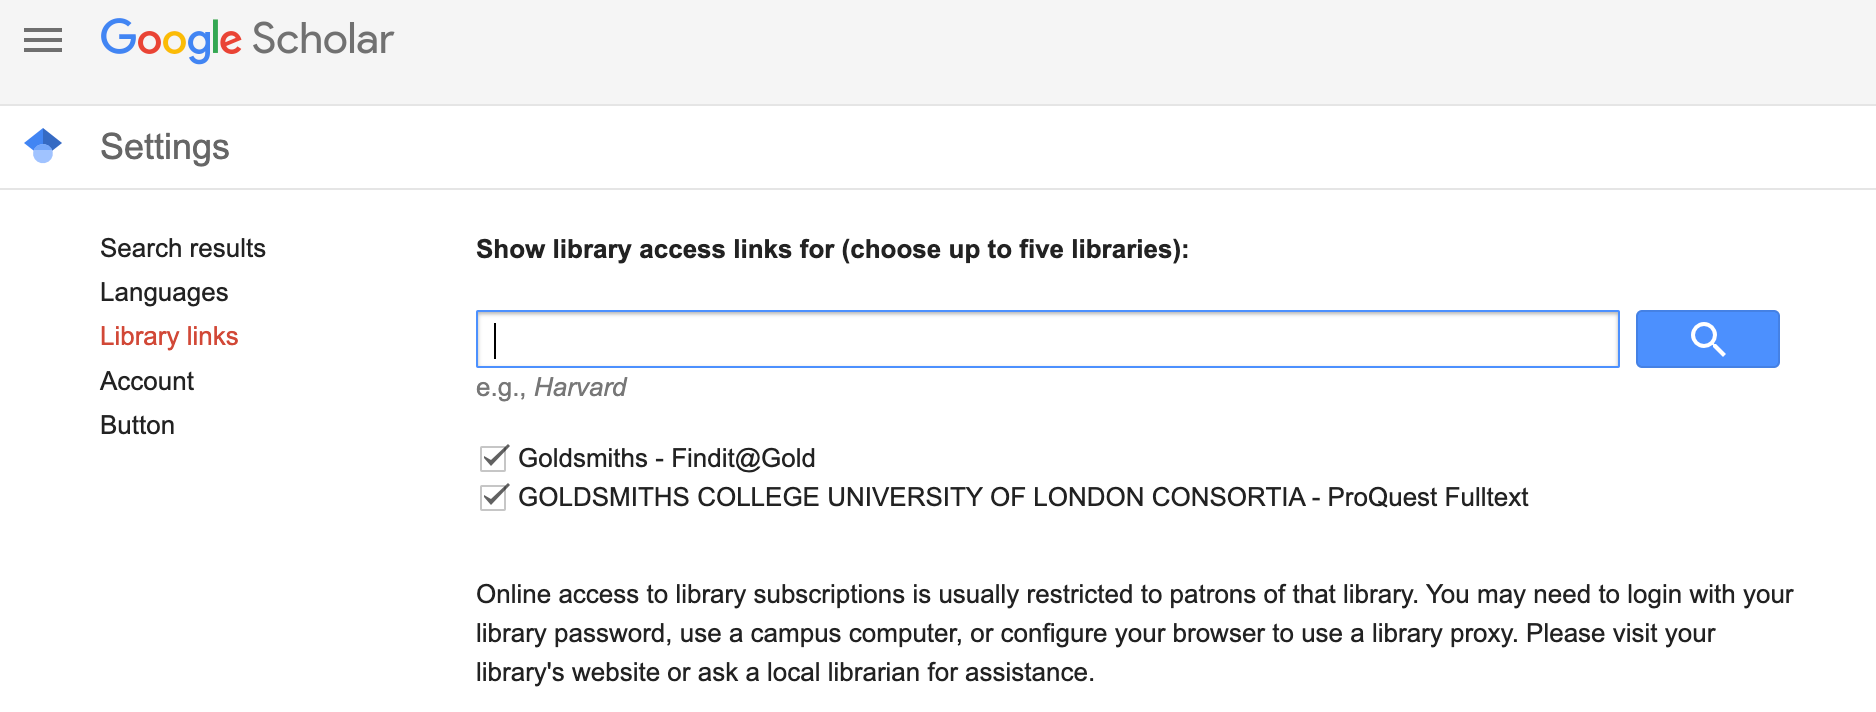
\includegraphics{images/paste-E9441F3F.png}


\includegraphics{images/paste-932C9782.png}

\end{tcolorbox}

\begin{center}\rule{0.5\linewidth}{0.5pt}\end{center}

\begin{tcolorbox}[enhanced jigsaw, arc=.35mm, opacitybacktitle=0.6, opacityback=0, leftrule=.75mm, colback=white, toprule=.15mm, rightrule=.15mm, coltitle=black, bottomrule=.15mm, bottomtitle=1mm, title=\textcolor{quarto-callout-tip-color}{\faLightbulb}\hspace{0.5em}{Tip Number 4}, colframe=quarto-callout-tip-color-frame, breakable, toptitle=1mm, titlerule=0mm, left=2mm, colbacktitle=quarto-callout-tip-color!10!white]

Strategic Searching \& Literature Management

\href{https://researchrabbitapp.com/home}{ResearchRabbit.ai} and
\href{https://www.zotero.org/}{Zotero}

Always keep your eyes open for

\href{https://www.annualreviews.org/journal/psych}{Annual Reviews of
Psychology}

Systematic Reviews and Meta-Analyses (Google Advanced Search!)

\end{tcolorbox}

\begin{center}\rule{0.5\linewidth}{0.5pt}\end{center}

\hypertarget{lets-get-going}{%
\section{Let's get going!}\label{lets-get-going}}

The link to our study for today is available on the VLE. It's called the
`Lie of the Land' study

\begin{center}\rule{0.5\linewidth}{0.5pt}\end{center}

2.5 Credits available today/this week

\hypertarget{the-study-link}{%
\subsection{The study link}\label{the-study-link}}

\url{https://goldpsych.eu.qualtrics.com/jfe/form/SV_ebMllxwNTfXHXRX}

\hypertarget{break}{%
\section{BREAK}\label{break}}

\hypertarget{littlemonkeylab}{%
\section{LittleMonkeyLab}\label{littlemonkeylab}}

\begin{longtable}[]{@{}
  >{\raggedright\arraybackslash}p{(\columnwidth - 0\tabcolsep) * \real{1.0000}}@{}}
\toprule\noalign{}
\endhead
\bottomrule\noalign{}
\endlastfoot
\#\# Some easy research! \\
\texttt{\{=html\}\ \textless{}iframe\ width="1280"\ height="720"\ src="https://learningonscreen.ac.uk/ondemand/embed/prog/11ED256E?bcast=127465838"\ title="Horizon:\ The\ Honesty\ Experiment"\ frameborder="0"\ allow="accelerometer;\ autoplay;\ clipboard-write;\ encrypted-media;\ gyroscope;\ picture-in-picture"\ allowfullscreen\textgreater{}\textless{}/iframe\textgreater{}}
\#\#
\href{https://learningonscreen.ac.uk/ondemand/embed/prog/11ED256E?bcast=127465838}{BBC
Horizon: The Honesty Experiment} \\
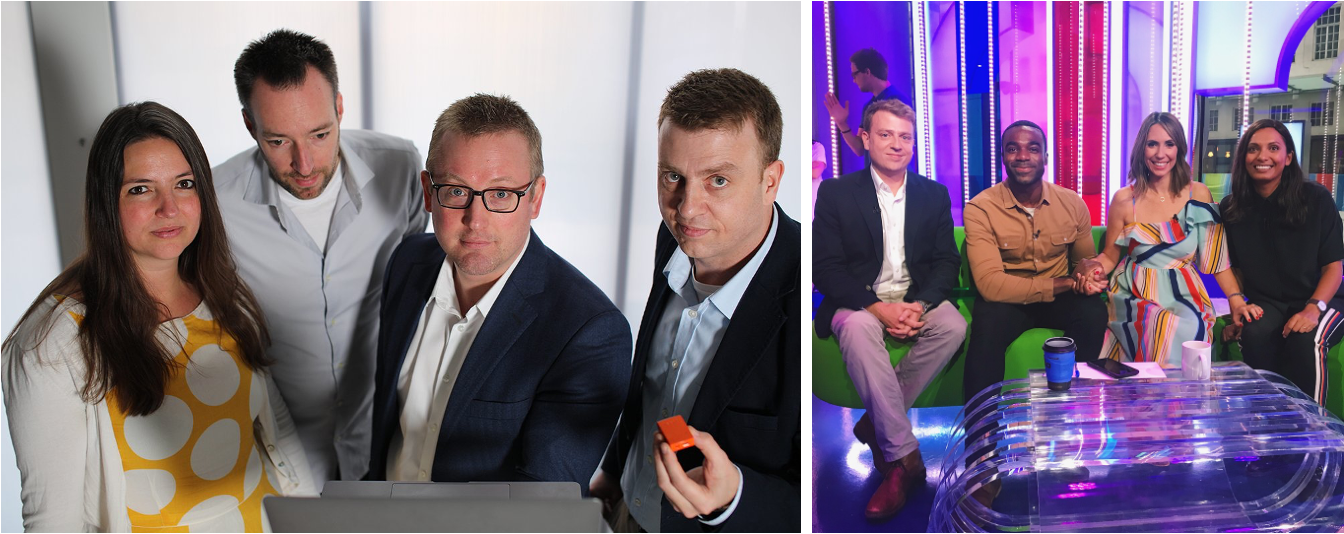
\includegraphics{images/paste-ABF42C39.png} \\
\end{longtable}


\includegraphics{images/paste-6B93028F.png}

\hypertarget{so-why-do-people-lie-levine2010d}{%
\subsection{So why do people lie? Levine et al.
(2010)}\label{so-why-do-people-lie-levine2010d}}

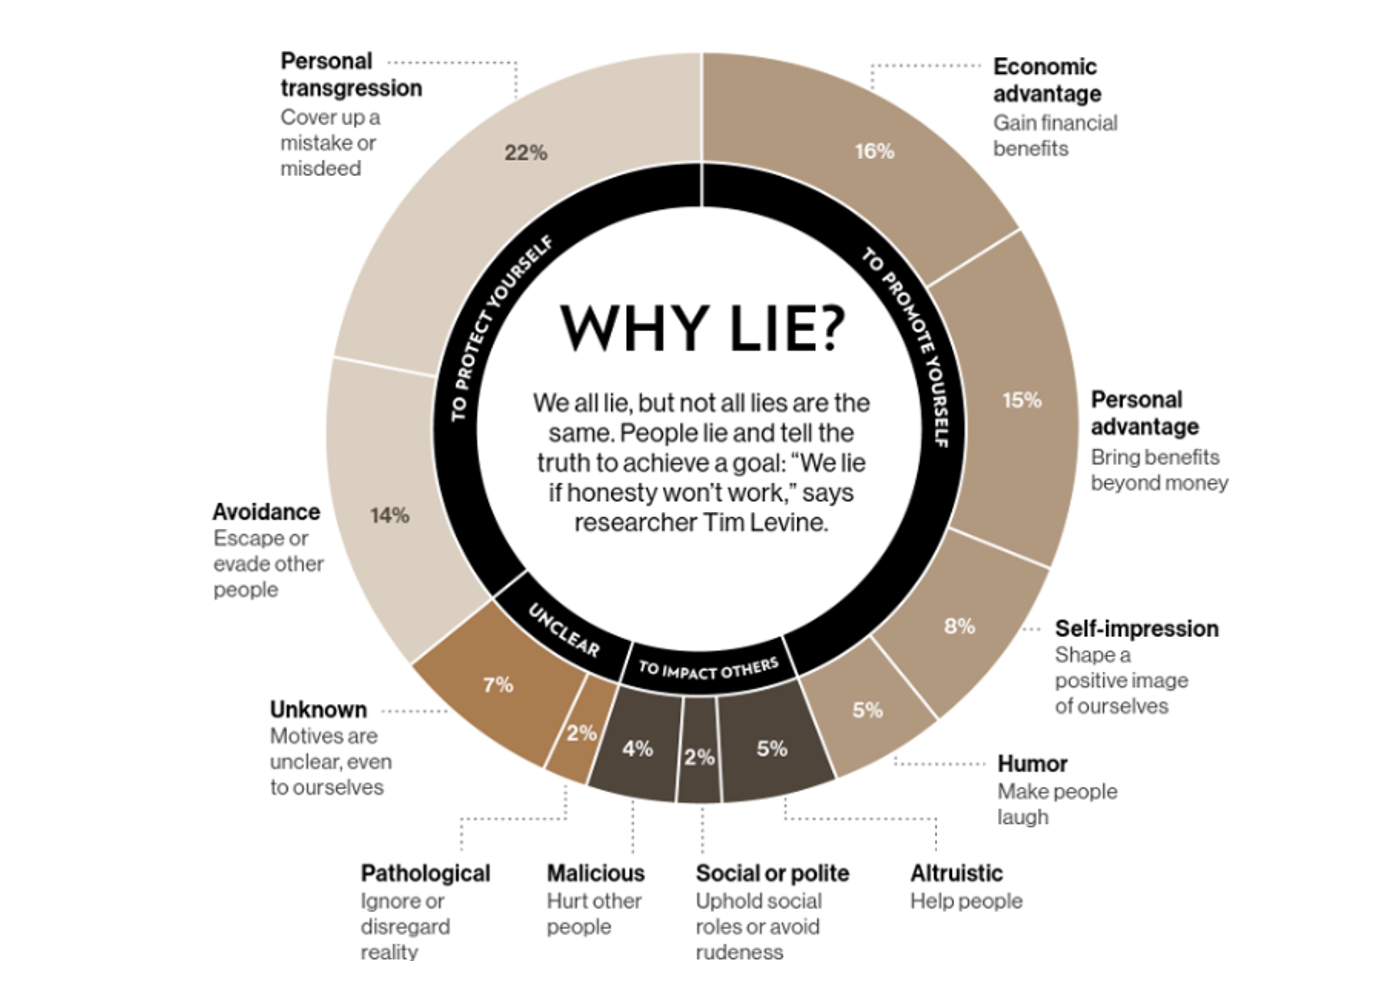
\includegraphics{images/paste-D0937F91.png}

\hypertarget{it-aint-that-bad-really}{%
\subsection{It ain't that bad really!}\label{it-aint-that-bad-really}}

Deception frequency is significantly correlated to neocortical volume
across species R. W. Byrne \& Corp (2004).

. . .

Evolution selects for more and more effective strategies of achieving
social success (including deception, manipulation, alliance formation,
exploitation of the expertise of others, etc.)

. . .

And for the ability to learn and use such strategies.

. . .

Social success translates into reproductive success!

\hypertarget{monkey-business-see-shultz2022}{%
\subsection{Monkey Business see Shultz \& Dunbar
(2022)}\label{monkey-business-see-shultz2022}}

. . .

\hfill\break
Observations of non-human behaviour of the type led scientists to
suggest a positive relationship between brain size and social group
size.

. . .

\hfill\break
A bigger brain seems to be found in more complex social environments.
But bigger brains are costly.

. . .

\hfill\break
There has to be a benefit to carrying around this big brain.

\hypertarget{the-dynamic-social-environment-see-whiten2018}{%
\subsection{The dynamic social environment see Whiten
(2018)}\label{the-dynamic-social-environment-see-whiten2018}}

. . .\\
The social world is very complex and the characters in this social world
are difficult to predict.

. . .\\
We usually operate within a status hierarchy which predetermines our
opportunities. Think of our cheeky little monkey. What did he want?

\begin{itemize}
\tightlist
\item
  Access to food
\item
  Access to shelter
\item
  Access to mates
\item
  Safety and Security of self and offspring
\end{itemize}

{Navigating the hierarchy successfully requires cooperation and
competition.}

\hypertarget{the-machiavellian-intelligence-hypothesis-byrne2018}{%
\subsection{The Machiavellian Intelligence Hypothesis (R. Byrne
(2018))}\label{the-machiavellian-intelligence-hypothesis-byrne2018}}

The Machiavellian Intelligence Hypothesis posits that social demands
have driven the evolution of the cognitive facilities humans employ to
navigate their social domain.

`Machiavellian' strategies, such as deception, interpersonal
manipulation, cooperation, and alliance formation allow individuals to
achieve higher social and reproductive success.

. . .\\

{Maybe it would help to be a bit more ``Machiavellian''?}

\hypertarget{but-how-can-we-possibly-measure-lie-frequency}{%
\subsection{But how can we possibly measure `Lie
Frequency'?}\label{but-how-can-we-possibly-measure-lie-frequency}}

Self- or other-report

Diary study (or similar)

Some kind of app?

Motion capture suits and TV cameras?

Experimental, lab-based research

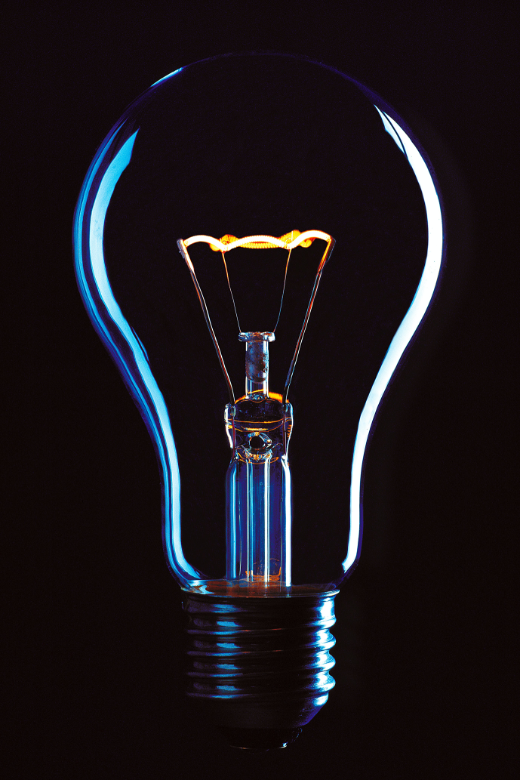
\includegraphics{images/paste-5E12FEC5.png}

\hypertarget{machiavellianism}{%
\subsection{Machiavellianism}\label{machiavellianism}}

. . .

Sensitive to social context, and will switch quickly between cooperation
and competition depending on utility

. . .

\hfill\break
Endorse emotional manipulation and use emotional skills to ingratiate

. . .

\hfill\break
Comprises a cynical view of human nature and interpersonal manipulation
tactics (perception of the world and behaviour)

\hypertarget{narcissism}{%
\subsection{Narcissism}\label{narcissism}}

. . .

Vain, `grandiose sense of self', with high levels of entitlement

. . .

\hfill\break
The Narcissist is unique and special

. . .

\hfill\break
Narcissists, as a result of being surrounded by `mere mortals' may show
reduced empathy for others and disregard their goals or status

. . .

\hfill\break
Narcissists maintain their grandiose sense of self by seeking out
praise, adoration, adulation and avoiding realistic feedback

Grandiose/Vulnerable distinction is starting to get hold.

\hypertarget{psychopathy}{%
\subsection{Psychopathy}\label{psychopathy}}

. . .

Manifest disregard for other people - Low empathy, disruptive behaviours
verging on bullying or sadism, deception thought to be a central
feature.

. . .

\hfill\break
Superficial charm and glibness. Erratic lifestyle factors and high
impulsivity. Extreme reward appetite and low fear of loss or punishment.
Often related to criminal activity.

. . .

\hfill\break
Boldness, Meanness, Disinhibition is the 3 Factor structure suggested by
the Triarchic Model (Patrick 2010, onwards)

\hypertarget{bonus-prize---sadism}{%
\subsection{Bonus prize - Sadism}\label{bonus-prize---sadism}}

. . .

As part of the Dark Tetrad, sadism is investigated in its subclinical
manifestation---\textbf{\emph{everyday sadism}}.

. . .

\hfill\break
When people enjoy watching violent movies or even playing violent games
as a social escape to manifest their sadistic traits it is referred to
as \textbf{\emph{vicarious sadism}}.

. . .

\hfill\break
There is sometimes an alternative aspect called \textbf{\emph{direct
sadism}}, but it is actually far too rare to be useful in most studies.

. . .

\hfill\break
In turn, higher scores in everyday sadism are associated with injuring
others verbally, physically, and/or psychologically, inspired by a
hedonic value of being cruel.

\hypertarget{for-a-comprehensive-overview}{%
\subsection{For a comprehensive
overview}\label{for-a-comprehensive-overview}}

Turi et al. (2022)

Bonfá-Araujo et al. (2022)

Levine (2022)

Denault et al. (2022)

\begin{center}\rule{0.5\linewidth}{0.5pt}\end{center}

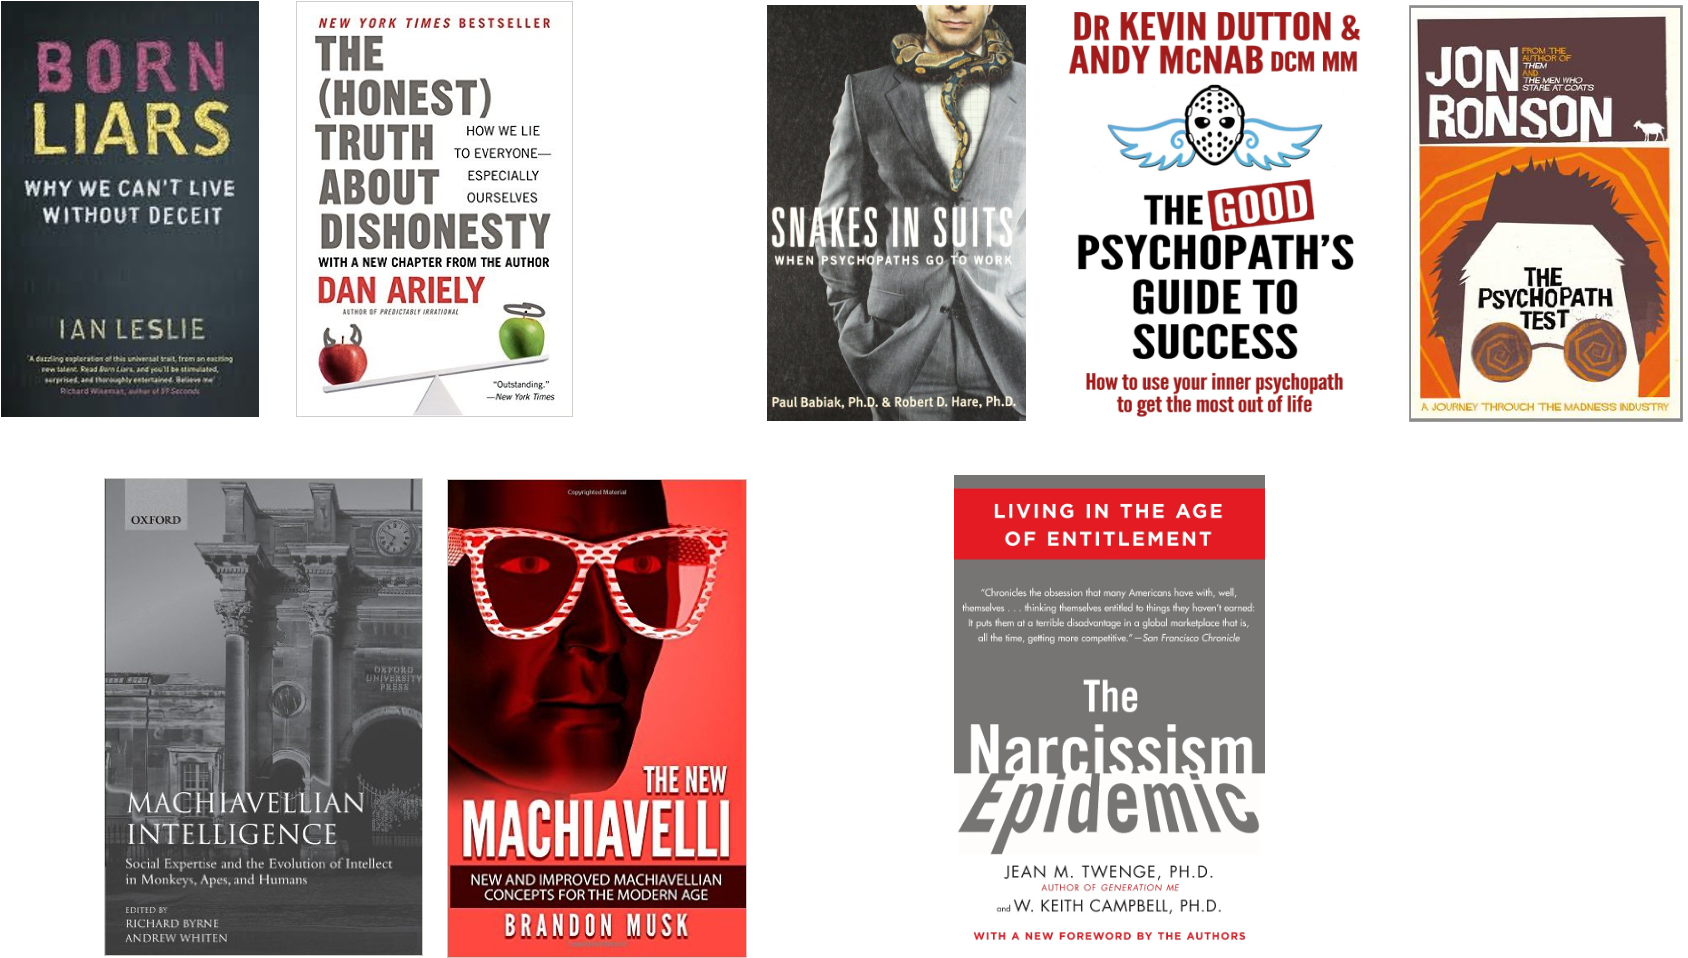
\includegraphics{images/paste-119912CF.png}

\hypertarget{the-target-paper-gunderson2022}{%
\subsection{The Target Paper Gunderson et al.
(2022)}\label{the-target-paper-gunderson2022}}

\url{https://hyp.is/L4vR9m9QEe2hne9nNT_AIg/link.springer.com/article/10.1007/s42761-022-00126-5}

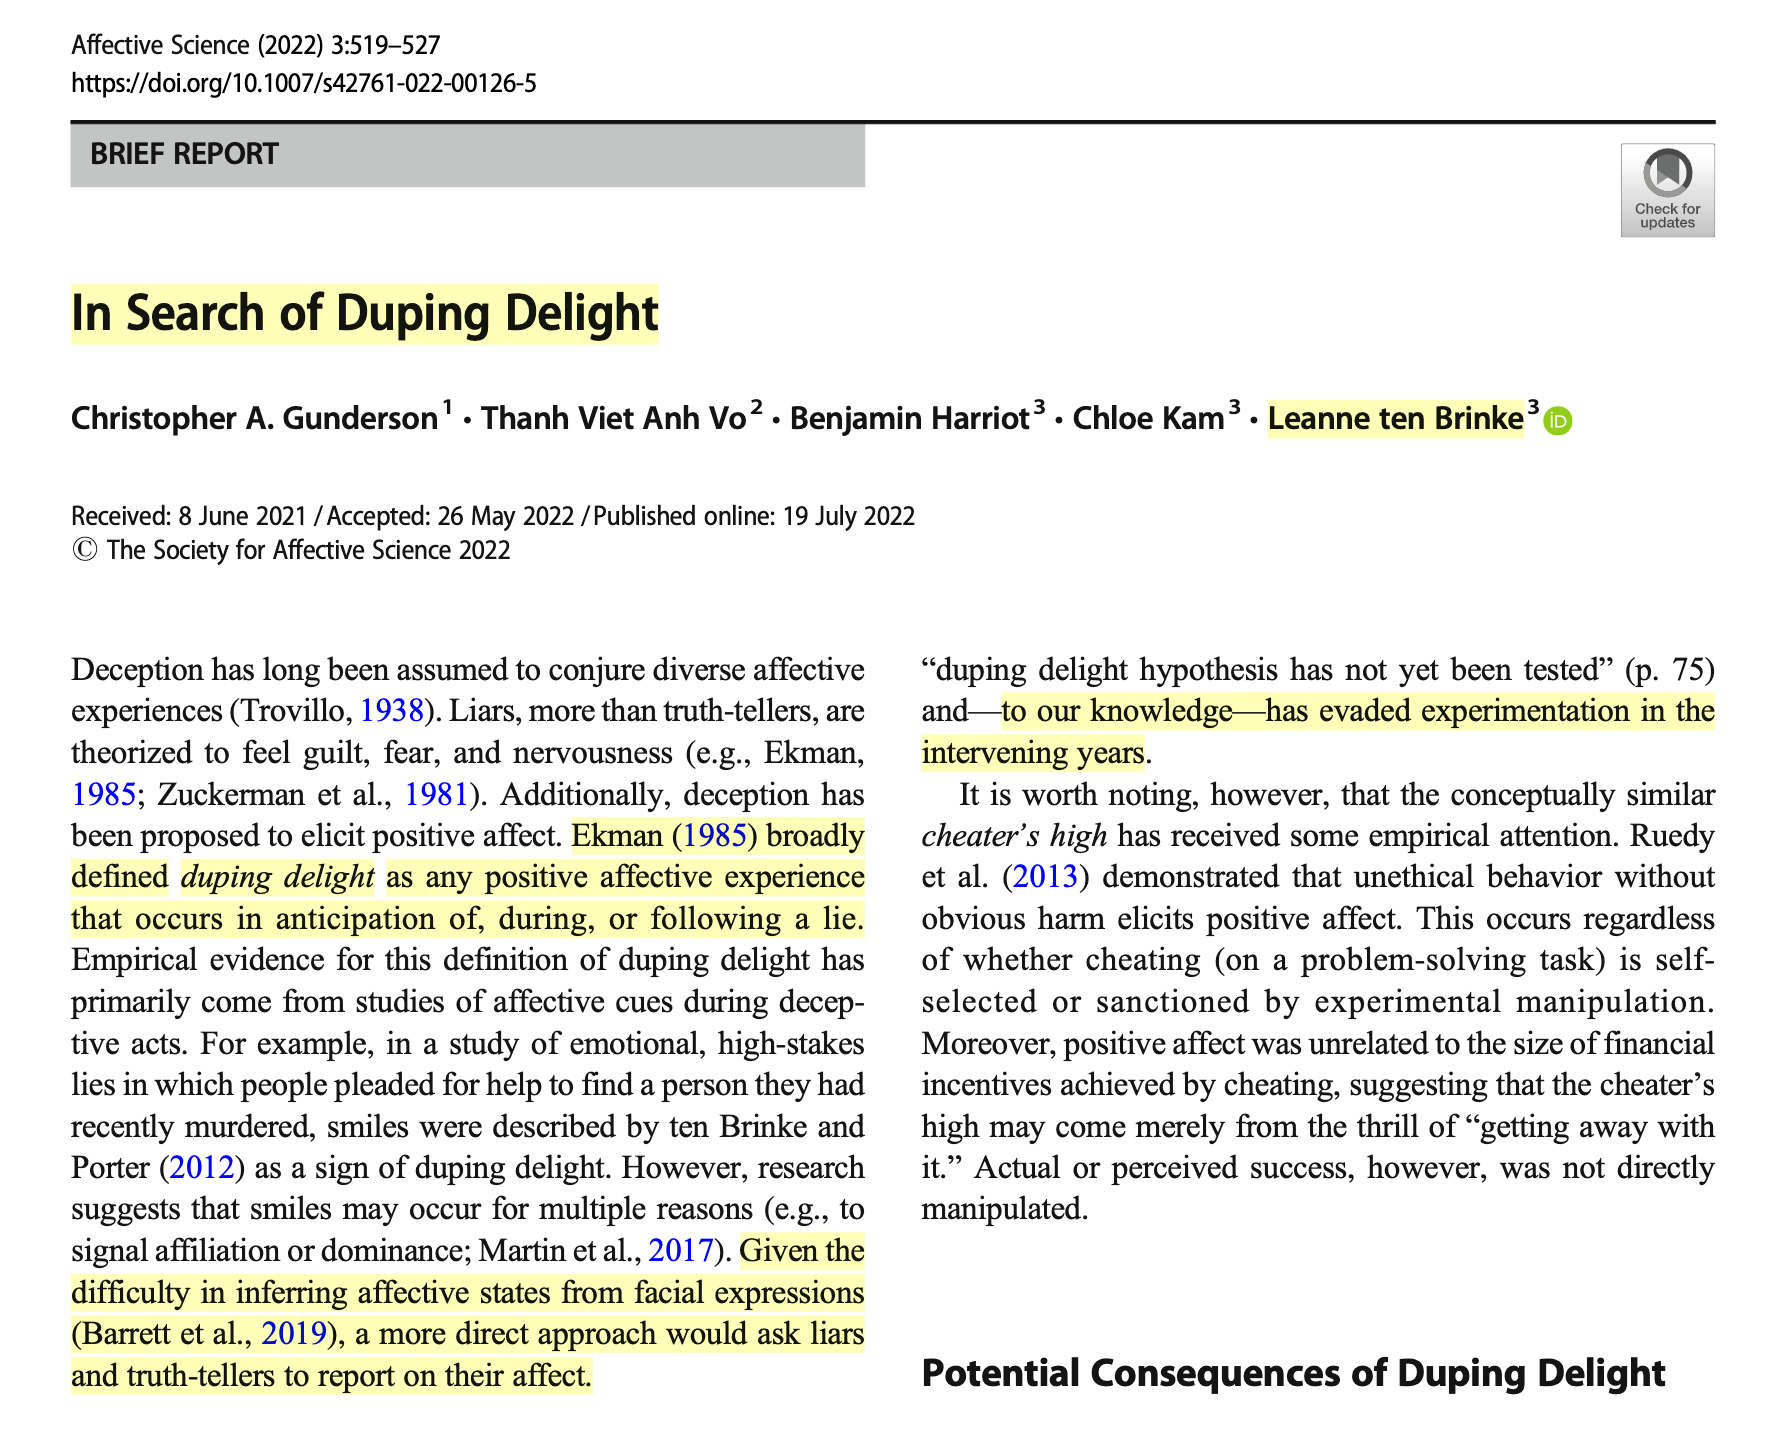
\includegraphics{images/paste-12B4ABA9.png}

\begin{center}\rule{0.5\linewidth}{0.5pt}\end{center}

\hypertarget{hypothes.is}{%
\subsection{Hypothes.is}\label{hypothes.is}}

hint: Sign up for a Hypothesis account (FREE)

Log in.

Then access the paper here:
\url{https://hyp.is/hvUM3m-KEe26bBOBEKqwUQ/link.springer.com/article/10.1007/s42761-022-00126-5}

\begin{figure}

{\centering 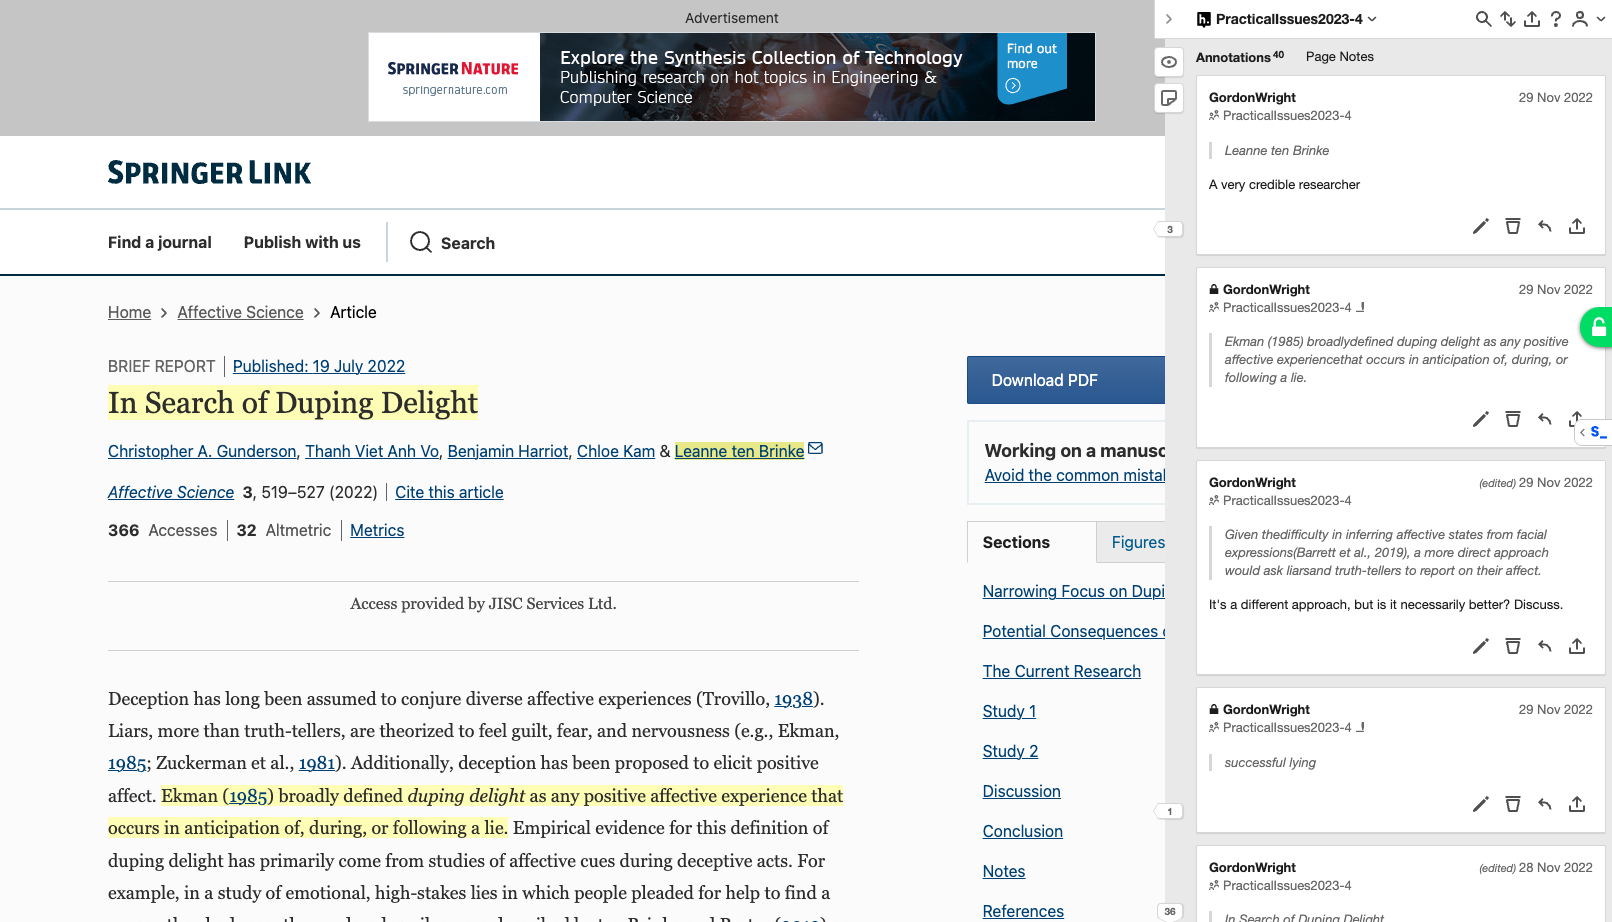
\includegraphics{images/Hypothesis@2x.png}

}

\caption{Hypothes.is}

\end{figure}

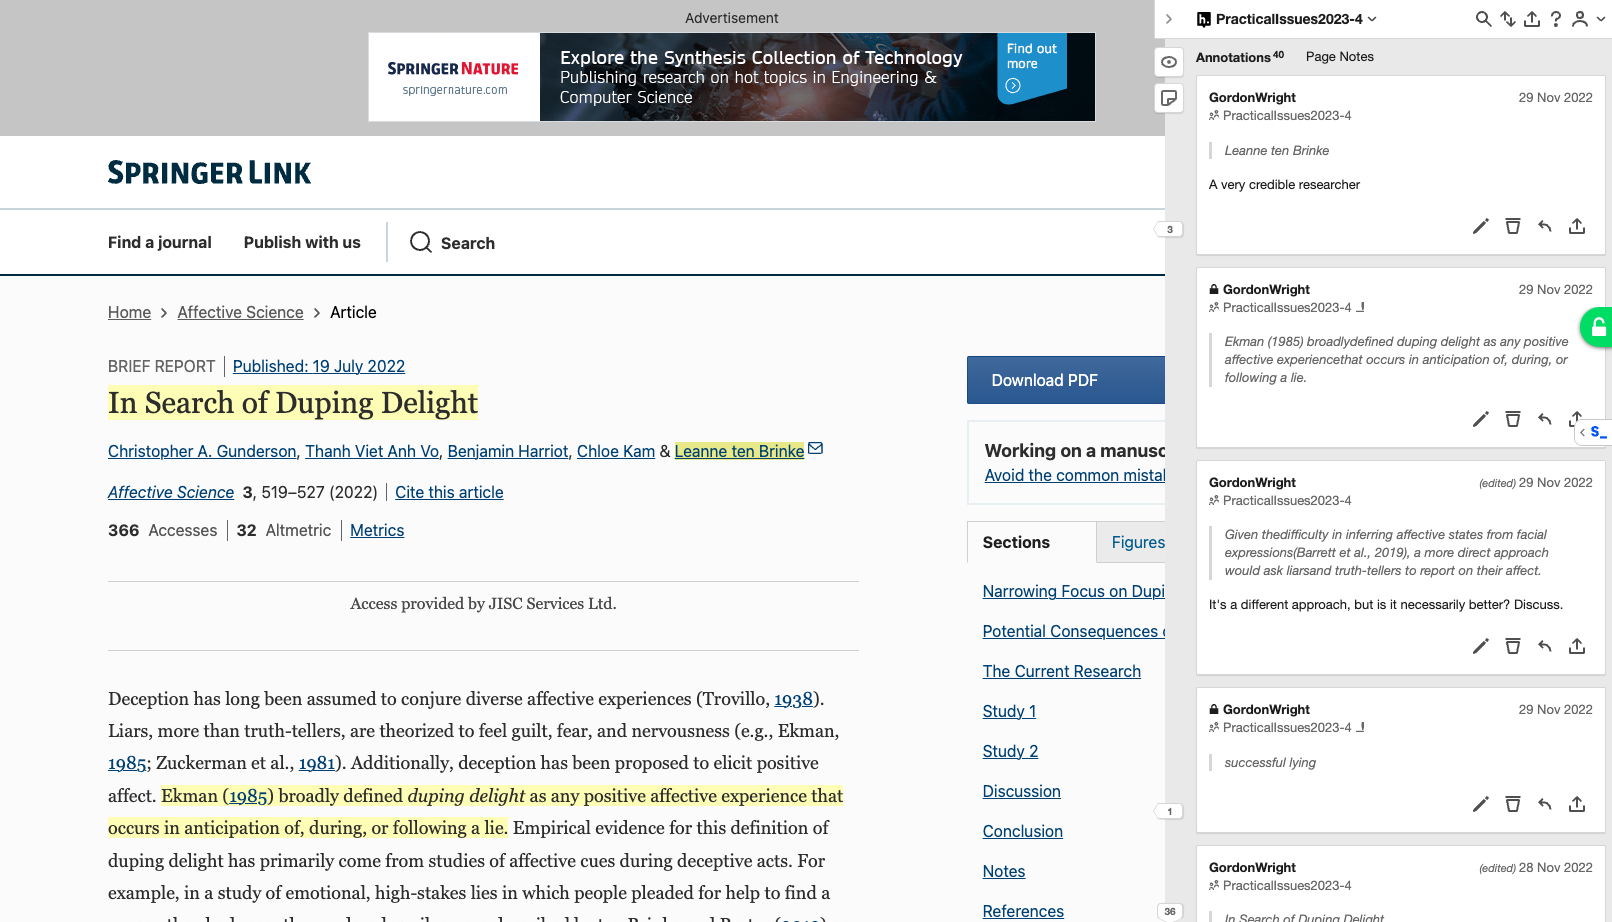
\includegraphics[width=1.5625in,height=0.125in]{images/Hypothesis@2x.png}

\hypertarget{so-lets-briefly-think-about-the-study}{%
\subsection{So let's briefly think about the
study}\label{so-lets-briefly-think-about-the-study}}

They `operationalised' deception in the following way:

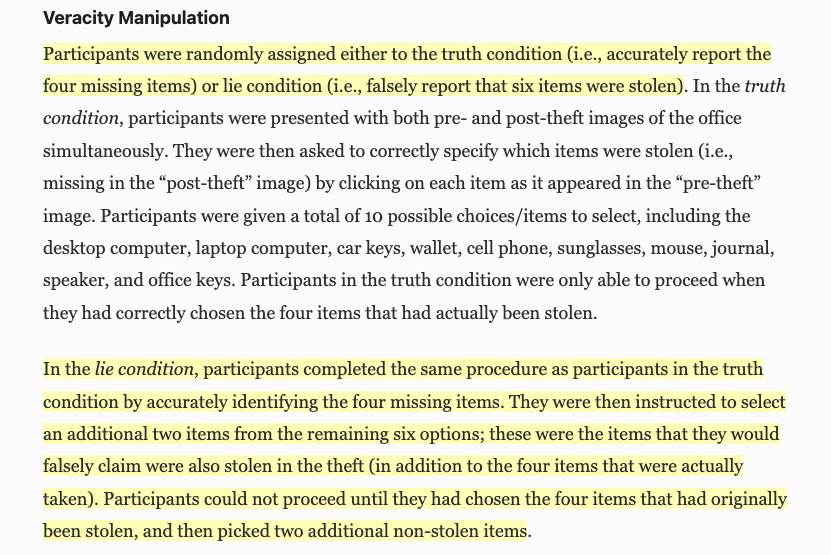
\includegraphics{images/Gunderson.png}

\hypertarget{they-measured-duping-delight}{%
\subsection{They measured `duping
delight'\ldots{}}\label{they-measured-duping-delight}}

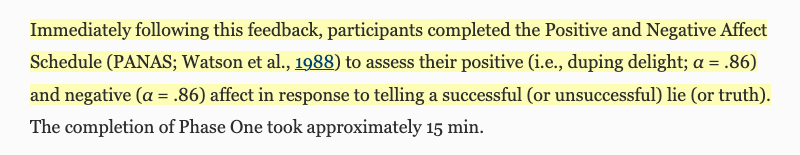
\includegraphics{images/PANAS@2x.png}

\hypertarget{does-that-satisfy-you}{%
\subsection{Does that satisfy you?}\label{does-that-satisfy-you}}

Is that a good way to measure an emotional reaction?

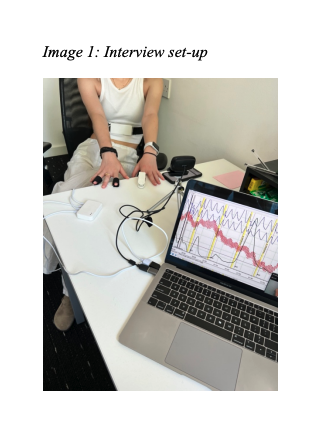
\includegraphics{images/Polygraph@2x.png}

\hypertarget{references}{%
\subsection*{References}\label{references}}
\addcontentsline{toc}{subsection}{References}

\hypertarget{refs}{}
\begin{CSLReferences}{1}{0}
\leavevmode\vadjust pre{\hypertarget{ref-bonfa-araujo2022}{}}%
Bonfá-Araujo, B., Lima-Costa, A. R., Hauck-Filho, N., \& Jonason, P. K.
(2022). Considering sadism in the shadow of the dark triad traits: A
meta-analytic review of the dark tetrad. \emph{Personality and
Individual Differences}, \emph{197}, 111767.

\leavevmode\vadjust pre{\hypertarget{ref-byrne2018}{}}%
Byrne, R. (2018). Machiavellian intelligence retrospective.
\emph{Journal of Comparative Psychology}.

\leavevmode\vadjust pre{\hypertarget{ref-byrne2004a}{}}%
Byrne, R. W., \& Corp, N. (2004). Neocortex size predicts deception rate
in primates. \emph{Proceedings of the Royal Society of London. Series B:
Biological Sciences Proc. R. Soc. Lond. B}, \emph{271}(1549),
1693--1699.

\leavevmode\vadjust pre{\hypertarget{ref-denault2022d}{}}%
Denault, V., Talwar, V., Plusquellec, P., \& Larivière, V. (2022). On
deception and lying: An overview of over 100 years of social science
research. \emph{Applied Cognitive Psychology}, \emph{36}(4), 805--819.

\leavevmode\vadjust pre{\hypertarget{ref-gunderson2022}{}}%
Gunderson, C. A., Vo, T. V. A., Harriot, B., Kam, C., \& Ten Brinke, L.
(2022). In search of duping delight. \emph{Affective Science},
\emph{3}(3), 519--527.

\leavevmode\vadjust pre{\hypertarget{ref-levine2022d}{}}%
Levine, T. R. (2022). Truth-default theory and the psychology of lying
and deception detection. \emph{Current Opinion in Psychology},
\emph{47}, 101380.

\leavevmode\vadjust pre{\hypertarget{ref-levine2010d}{}}%
Levine, T. R., Kim, R. K., \& Hamel, L. M. (2010). People lie for a
reason: Three experiments documenting the principle of veracity.
\emph{Communication Research Reports}, \emph{27}(4), 271--285.

\leavevmode\vadjust pre{\hypertarget{ref-shultz2022}{}}%
Shultz, S., \& Dunbar, R. I. (2022). Socioecological complexity in
primate groups and its cognitive correlates. \emph{Philosophical
Transactions of the Royal Society B}, \emph{377}(1860), 20210296.

\leavevmode\vadjust pre{\hypertarget{ref-turi2022a}{}}%
Turi, A., Rebeleș, M.-R., \& Visu-Petra, L. (2022). The tangled webs
they weave: A scoping review of deception detection and production in
relation to dark triad traits. \emph{Acta Psychol (Amst)}, \emph{226},
103574.

\leavevmode\vadjust pre{\hypertarget{ref-whiten2018}{}}%
Whiten, A. (2018). Social, machiavellian and cultural cognition: A
golden age of discovery in comparative and evolutionary psychology.
\emph{Journal of Comparative Psychology}.

\end{CSLReferences}



\end{document}
